%%%%%%%%%%%%%%%%%%%%%%%%%%%%%%%%%%%%%%%%%
% Journal Article
% LaTeX Template
% Version 1.4 (15/5/16)
%
% This template has been downloaded from:
% http://www.LaTeXTemplates.com
%
% Original author:
% Frits Wenneker (http://www.howtotex.com) with extensive modifications by
% Vel (vel@LaTeXTemplates.com)
%
% License:
% CC BY-NC-SA 3.0 (http://creativecommons.org/licenses/by-nc-sa/3.0/)
%
%%%%%%%%%%%%%%%%%%%%%%%%%%%%%%%%%%%%%%%%%

%----------------------------------------------------------------------------------------
%	PACKAGES AND OTHER DOCUMENT CONFIGURATIONS
%----------------------------------------------------------------------------------------

\documentclass[twocolumn]{article}

\usepackage[sc]{mathpazo} % Use the Palatino font
\usepackage[T1]{fontenc} % Use 8-bit encoding that has 256 glyphs
\linespread{1.05} % Line spacing - Palatino needs more space between lines
\usepackage{microtype} % Slightly tweak font spacing for aesthetics

\usepackage[english]{babel} % Language hyphenation and typographical rules

\usepackage[hmarginratio=1:1,top=32mm,columnsep=20pt]{geometry} % Document margins
\usepackage[hang, small,labelfont=bf,up,textfont=it,up]{caption} % Custom captions under/above floats in tables or figures
\usepackage{booktabs} % Horizontal rules in tables

\usepackage{lettrine} % The lettrine is the first enlarged letter at the beginning of the text

\usepackage{enumitem} % Customized lists
\setlist[itemize]{noitemsep} % Make itemize lists more compact

\usepackage{abstract} % Allows abstract customization
\renewcommand{\abstractnamefont}{\normalfont\bfseries} % Set the "Abstract" text to bold
\renewcommand{\abstracttextfont}{\normalfont\small\itshape} % Set the abstract itself to small italic text

\usepackage{titlesec} % Allows customization of titles
\renewcommand\thesection{\Roman{section}} % Roman numerals for the sections
\renewcommand\thesubsection{\roman{subsection}} % roman numerals for subsections
\titleformat{\section}[block]{\large\scshape\centering}{\thesection.}{1em}{} % Change the look of the section titles
\titleformat{\subsection}[block]{\large}{\thesubsection.}{1em}{} % Change the look of the section titles

\usepackage{fancyhdr} % Headers and footers
\pagestyle{fancy} % All pages have headers and footers
\fancyhead{} % Blank out the default header
\fancyfoot{} % Blank out the default footer
\fancyhead[C]{Semantic Parsing with a domain Ontology} % Custom header text
\fancyfoot[C]{\thepage} % Custom footer text

\usepackage{titling} % Customizing the title section

\usepackage{graphicx}

\usepackage{hyperref} % For hyperlinks in the PDF

%----------------------------------------------------------------------------------------
%	TITLE SECTION
%----------------------------------------------------------------------------------------

\setlength{\droptitle}{-4\baselineskip} % Move the title up

\pretitle{\begin{center}\Huge\bfseries} % Article title formatting
\posttitle{\end{center}} % Article title closing formatting
\title{Semantic Parsing with a domain Ontology} % Article title
\author{%
\textsc{Corentin Dumont} \\[1ex] % Your name
\normalsize Tohoku University \\ % Your institution
\normalsize \href{corentin-d@ecei.tohoku.ac.jp}{corentin-d@ecei.tohoku.ac.jp} % Your email address
\and % Uncomment if 2 authors are required, duplicate these 4 lines if more
\textsc{Ran Tian} \\[1ex] % Second author's name
\normalsize Tohoku University \\ % Second author's institution
\normalsize \href{tianran@ecei.tohoku.ac.jp}{tianran@ecei.tohoku.ac.jp} % Second author's email address
\and % Uncomment if 2 authors are required, duplicate these 4 lines if more
\textsc{Kentaro Inui} \\[1ex] % Second author's name
\normalsize Tohoku University \\ % Second author's institution
\normalsize \href{inui@ecei.tohoku.ac.jp}{inui@ecei.tohoku.ac.jp} % Second author's email address
}
%\date{\today} % Leave empty to omit a date
\date{}
\renewcommand{\maketitlehookd}{%
\begin{abstract}
\noindent Using restricted domains in question answering (QA) allows to build an ontology of the domain that can be used with by a semantic parser to improve the performance of a QA system. However, building an ontology and a semantic parser can be costly and usually require a large amount of annotated data that may not be available for specific domains. Our work is a case study on how to build a semantic parser and a domain ontology with very low resource for the video game Minecraft.\\
We show that the creation of a semantic parser and the ontology it is based on can be done with a very low amount of expert manual annotations, facilitated by the use of automatically collected data from the web, and that fairly good performance can be obtained.
Thus, as a contribution, this case study is a first step in solving the common problem of building a QA system in a restricted domain from very low resource and low manual effort.
\end{abstract}
}

%----------------------------------------------------------------------------------------

\begin{document}

% Print the title
\maketitle

%----------------------------------------------------------------------------------------
%	ARTICLE CONTENTS
%----------------------------------------------------------------------------------------

\section{Introduction}

%The initial motivation of this work is to improve the interaction between the players and Non-Player Characters (NPCs) in video games. As in Figure~\ref{currentInteraction}, in current video games, interaction between the player and the NPCs is very limited in the sense that the player cannot ask his own questions. Indeed, the game will often propose several possible questions or choices to the player, who can only choose among them.\\
%\begin{figure}[!ht]
%	\centering 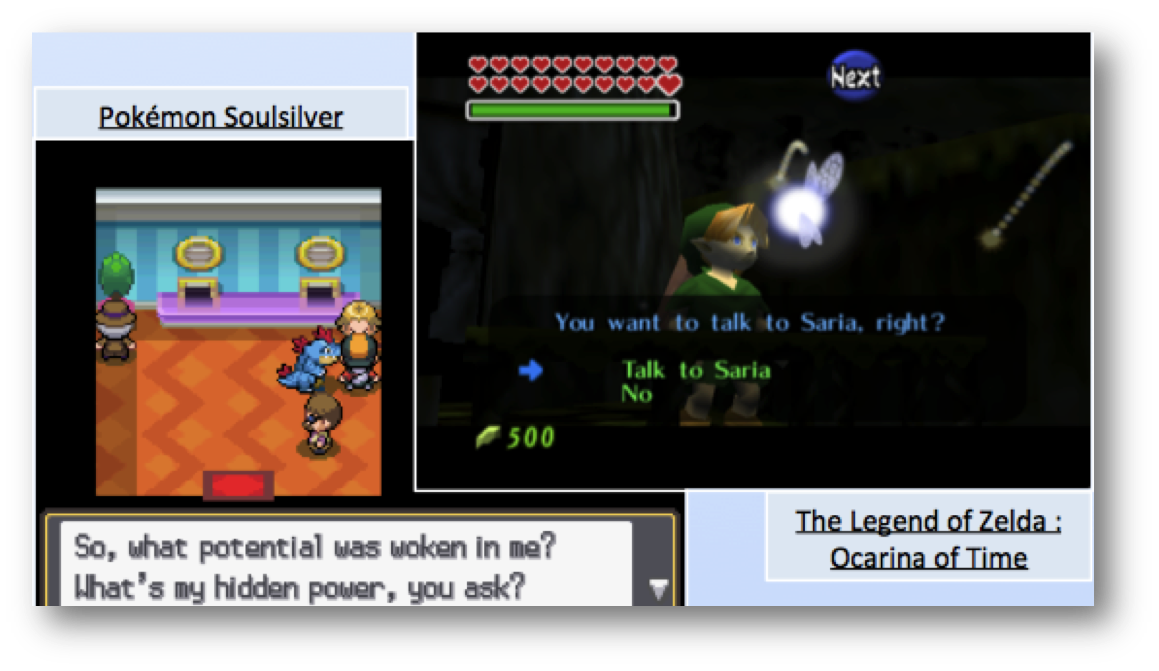
\includegraphics[width=0.9\linewidth]{Figures/Intro_Conclusion/currentInteraction.png}
%	\caption{\label{currentInteraction}Interaction between players and NPCs in current video games}
%\end{figure}
%Our final goal is to develop a natural language question answering system that would make possible a real interaction between the player and the NPCs. Such a system, as shown in Figure~\ref{goal}, would allow the player to ask about anything in English about the content of the game, and make the NPCs able to answer in natural English to any question of the player as long as it is about the content of the game.\\
%\begin{figure}[!ht]
%	\centering 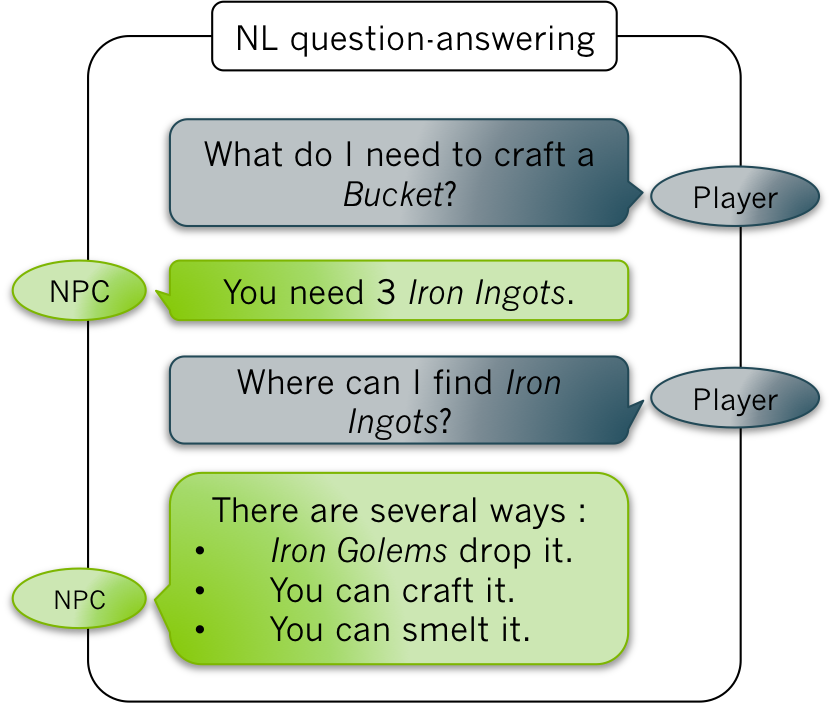
\includegraphics[width=0.7\linewidth]{Figures/Intro_Conclusion/goal.png}
%	\caption{\label{goal}The final goal of our work, a natural language QA system}
%\end{figure}
%Unlike many QA systems that are designed to answer real world questions \cite{berant2014semantic,yao2015lean}, the final goal of this research is to build a system that can answer questions using the logic specific to the game, which may not be identical to the logic in the real world. For our study, we choose a popular game called Minecraft, whose openness provides a great liberty for players, which guarantees a large number of possible questions to ask about the game, and yet the presence of a specific logic that limits the actions of players. We are interested in this problem setting because it provides a testbed for combining Natural Language Processing with advanced logical inference techniques.\\
%Our final system should be able to access knowledge about the content of the game, so we need to collect this knowledge. It should also understand the content of this knowledge and the players' questions in order to construct a relevant answer, so we need to build a semantic parser that will extract the meaning from English sentences by finding the important instances and the relations that link these instances together. Finally, it has to answer the questions by constructing relevant answers from the knowledge it has about the game using logical inference techniques.\\
%As a whole, our work is a case study on how to build a Semantic Parser (and in the end, a complete Question Answering system) from very low resource in the restricted domain of a video game.

%------------------------------------------------

\section{Ontology}

In this study, we use the ontology for Minecraft described in \cite{dumont2016ontology}. In its current state, this ontology defines two types of classes to represent the instances in Minecraft and the relations that links these instances together.\\
The \textbf{Instance classes} regroup Minecraft Entities and Events (Figure~\ref{entitiesAndEvents}), and the ontology defines the list of 496 Entity classes and their hierarchy and 12 Event classes.\\
The \textbf{Relation classes} represent a link between two instances. The ontology defines the list of 54 Relation classes and the constraints that define what Instances classes can be linked using each Relation class.

\begin{figure}[t]
   \centering 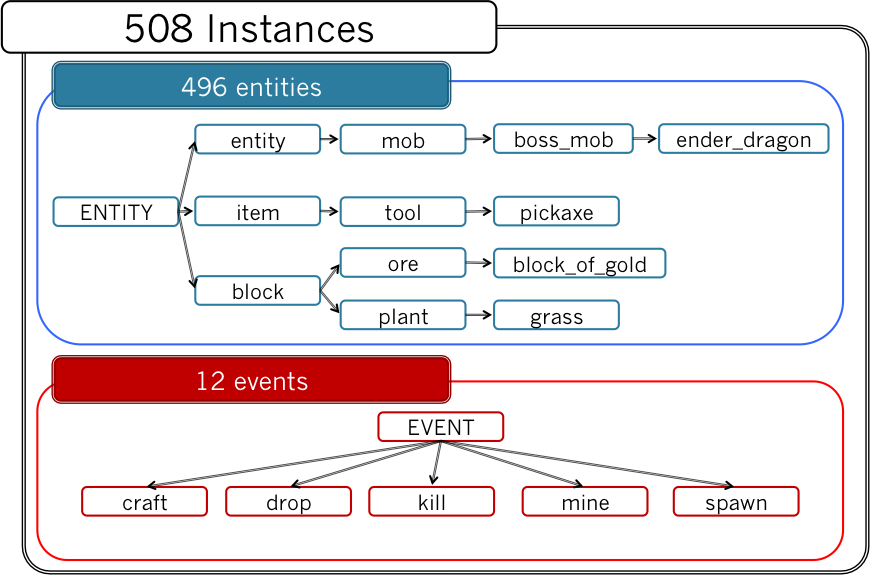
\includegraphics[width=\linewidth]{Figures/Knowledge/entitiesAndEvents.png}
   \caption{\label{entitiesAndEvents} Instances of the Ontology}
\end{figure}

%------------------------------------------------

\section{Training dataset}

\begin{table*}[t]
\center
\begin{tabular}{c||c|c|c||c|c|c}
	 & \multicolumn{3}{c||}{instance samples} & \multicolumn{3}{c}{relation samples} \\
	 & positive & negative & total & positive & negative & total \\ \hline \hline
	manual & 142 & 159 & 301 & 266 & 219 & 485\\ \hline
	automatic & 6471 & & 6471 & & & \\ \hline
	crowd-sourcing & & & & 158 & 52 & 210\\ \hline \hline
	total & 6613 & 159 & \textbf{6772} & 324 & 271 & \textbf{695}
\end{tabular}
\caption{\label{dataset} Training dataset}
\end{table*}

\begin{figure*}[t]
   \centering 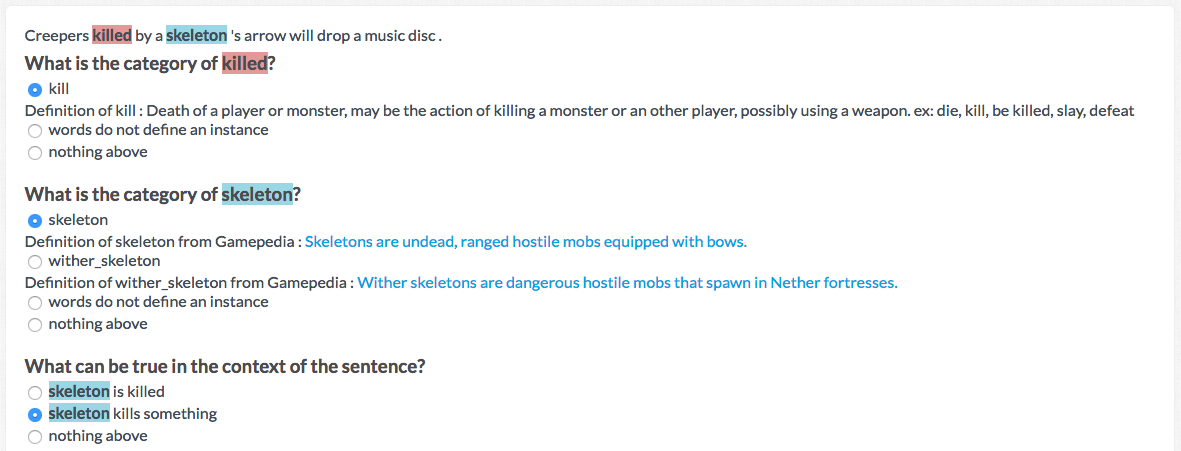
\includegraphics[width=\linewidth]{Figures/Semantic_Parsing/crowdSourcing.png}
   \caption{\label{crowdSourcing} Example of crowd-sourcing annotation with CrowdFlower}
\end{figure*}

In order to train a semantic parser for Minecraft to recognize instances and relations in sentences, we built a training dataset by annotating instances and relations in sentences about Minecraft (Table~\ref{dataset}). This annotation was done on simple sentences that were taken from a knowledge corpus described in \cite{dumont2016question}, extracted from 3 different wiki-like websites about Minecraft.\\
To do this annotation more easily, we developed a specific annotation tool that integrates the ontology. As the annotation tool can the ontology, the annotator is proposed the different possible labels, which simplify the annotation process and ensure that the annotations respect the ontology constraints. Using this tool, we manually annotated 301 samples of instances (142 positive examples and 159 negative examples) and 485 samples of relations (266 positive examples and 219 negative examples).\\
Furthermore, we also created 6471 automatic samples of instances (positive examples only) from the anchors contained in the knowledge corpus, which link a fragment of text to the title of an other page. When the title of the page pointed by a hyperlink can be identify as the name of an instance class in the ontology, the fragment of text that holds the hyperlink becomes a positive example for this instance class, and is added to the training dataset.\\
If we have been able to generate automatically a lot of instances samples, we do not dispose of such a way to generate easily relation samples. One solution is to use crowd-sourcing to obtain cheap annotations made by non-expert annotators on the web. However, annotating relations between two instances in a text is a difficult task that requires knowing the characteristics of the ontology. To make non-expert annotators to realize such an annotation, for each relation sample to be annotated, we automatically list all possible relations respecting the ontology's constraints and, for each possible relation, generate a proposition in English that is easy to understand for human annotators and asserts that the relation is true in the context of the sentence. Then, we ask annotators to choose the only proposition that is true (the ontology is designed in a way that there is always at most only one relation between two instances). Each sample is annotated by 5 different annotators, and the most reliable answer is added to the training dataset. We obtained 210 distinct relation samples (158 positive examples, and 52 negative examples) for 9 different relation classes. This crowd-sourcing has been realized with the CrowdFlower platform\footnote{\href{http://www.crowdflower.com/}{www.crowdflower.com}} (example in Figure~\ref{crowdSourcing}).

%------------------------------------------------

\section{Semantic Parsing}

In the context of our study, \textbf{semantic parsing} is a process that take a sentence as input and outputs a knowledge graph that represents the meaning of the sentence (see Figure~\ref{semanticParsingFigure}).

\begin{figure}[t]
	\centering 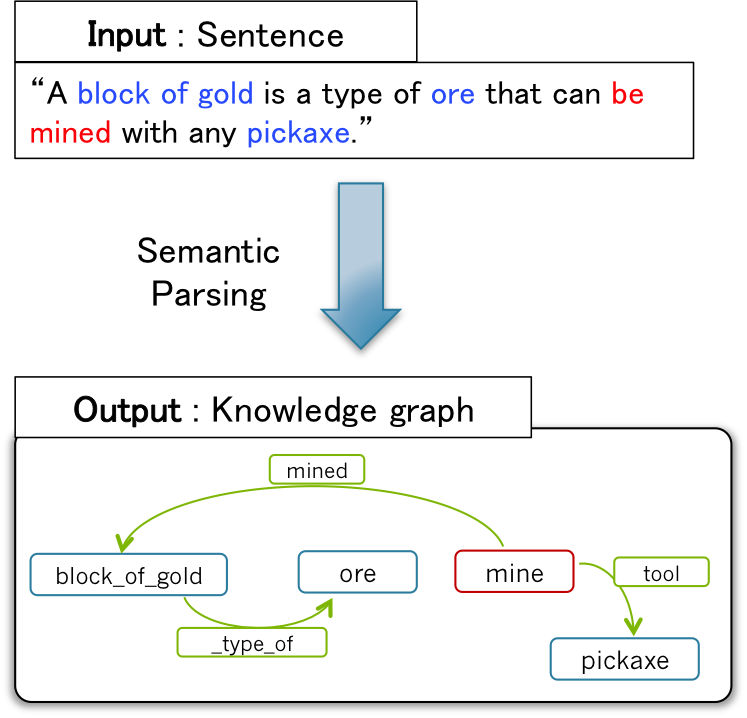
\includegraphics[width=\linewidth]{Figures/Semantic_Parsing/semanticParsingFigure.png}
	\caption{\label{semanticParsingFigure}Semantic Parsing}
\end{figure}

The knowledge graph is composed of instances (the nodes) and relations (the edges) that belong to the ontology that we defined previously.\\
The knowledge graph is constructed in two steps, the instance classification that generates the nodes, and the relation classification that generates the edges.\\
There is an other process called \textbf{syntactic parsing} that, like semantic parsing, generates an output graph (the syntactic tree, see Figure~\ref{syntacticTree}) from an input sentence, but, contrary to semantic parsing, this graph does not represent the meaning of the sentence but its syntax. Nodes are the words of the sentence, and edges are the syntactic dependencies between these words.

\begin{figure}[t]
	\centering 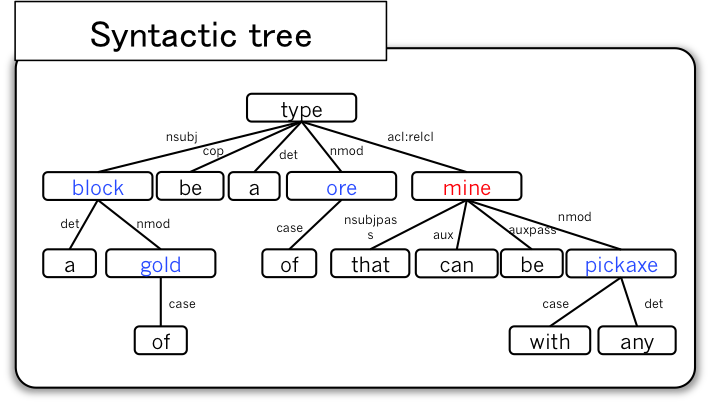
\includegraphics[width=\linewidth]{Figures/Semantic_Parsing/syntacticTree.png}
	\caption{\label{syntacticTree}Syntactic tree of the sentence ``A block a gold is a type of ore that can be mined with any pickaxe''}
\end{figure}

We can notice a similarity between the knowledge graph and the syntactic tree. Thus, our idea was to use the information contained in the syntactic tree as a base for the semantic parsing. In particular, using the words (nodes of the syntactic tree) in the instance classification step, and the syntactic dependencies (edges of the syntactic tree) in relation classification step.\\
The syntactic parsing process does not depend on a domain ontology; it has been largely studied in the past and performing syntactic parsers have been released by NLP researchers \cite{chen2014fast,andor2016globally}. So we can easily apply existing syntactic parsers to our work, and use syntactic trees in our semantic parsing.

\subsection{Instance classification}

Instance classification is the classification of a phrase (a group of words) into an instance class from the ontology. So we need to extract features to classify from phrases. Word embedding has been shown to produce non-sparse and effective features to represent the meaning of words \cite{mikolov2013efficient}.

\subsubsection{Word Embedding}

Therefore, we trained a word embedding model using as a training corpus the knowledge corpus extracted before, which is a corpus of words sequences specific to Minecraft, with the skip-gram model of the Word2Vec library \cite{mikolov2013distributed}. We obtain a model that produce similar vectors for words with a similar meaning in the context of Minecraft.

\begin{figure}[t]
   \centering 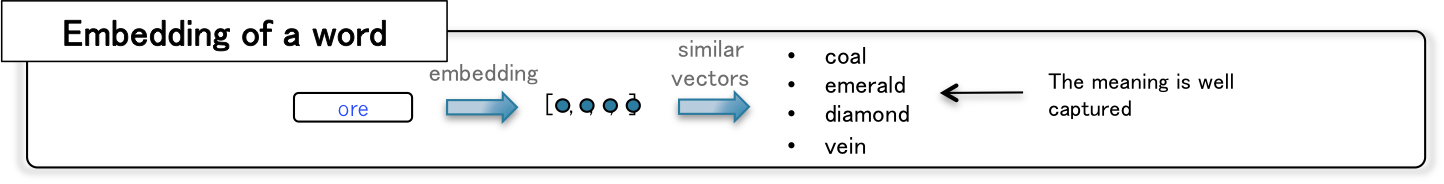
\includegraphics[width=\linewidth]{Figures/Semantic_Parsing/wordEmbedding.png}
   \caption{\label{wordEmbedding} Embedding of the word ``ore''}
\end{figure}

Then, the embedding representation of a phrase using our Word2Vec model is calculated as the average vector of the embedding representation of all words in the phrase.\\
The challenging point is to create, from a word embedding model, a model that embed correctly the meaning of a phrase. Our Word2Vec based phrase embedding model does not include the different importance of the words in natural language (e.g. in ``a baby villager'', the word ``villager'' is more important to catch the meaning of the instance described than the word ``baby''). This difference between the importances of each word in a phrase is visible in the syntactic tree that represents this phrase. The most important word is the root of the tree, which is specified by its children nodes, and deepest nodes have least importance.\\
In other words, it could be interesting to include, in the embedding of a phrase, the syntactic pattern followed by the words, which is a quite difficult task \cite{takase2016modeling}.
However, more specifically, we can keep an information on the syntactic relations between the words by using the VecDCS library \cite{tian2016learning}. In this method, the embedding representation of a phrase is calculated using the DCS tree representation of the phrase that can be obtained from the syntactic tree (Figure~\ref{dcsTree}).

\begin{figure}[t]
   \centering 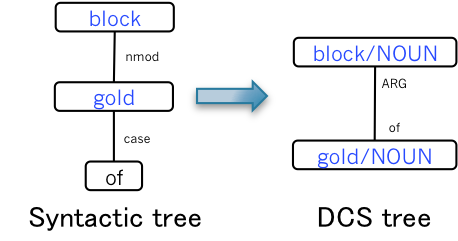
\includegraphics[width=\linewidth]{Figures/Semantic_Parsing/dcsTree.png}
   \caption{\label{dcsTree} DCS tree of the phrase ``block of gold''}
\end{figure}

And the VecDCS embedding of the phrase can be calculated from the individual embedding vectors of the different nodes of the DCS tree by the formula given in Figure~\ref{vecDCSFormula}.

\begin{figure}[t]
   \centering 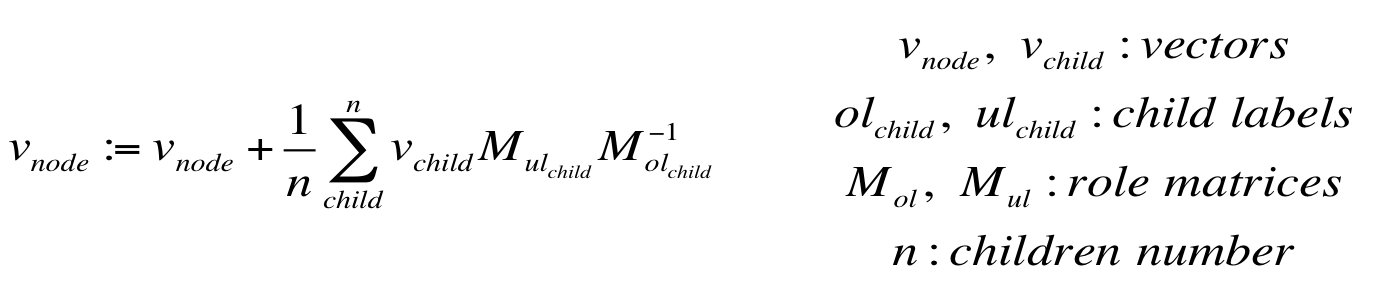
\includegraphics[width=\linewidth]{Figures/Semantic_Parsing/vecDCS.png}
   \caption{\label{vecDCSFormula} Formula of the VecDCS embedding vector of a syntactic sub-tree}
\end{figure}

Therefore, we also trained a VecDCS model for Minecraft, using the extracted knowledge corpus.
We dispose of two different phrase embedding models that can be use to produce features for instance classification (Word2Vec model and VecDCS model).

\begin{figure}[t]
   \centering 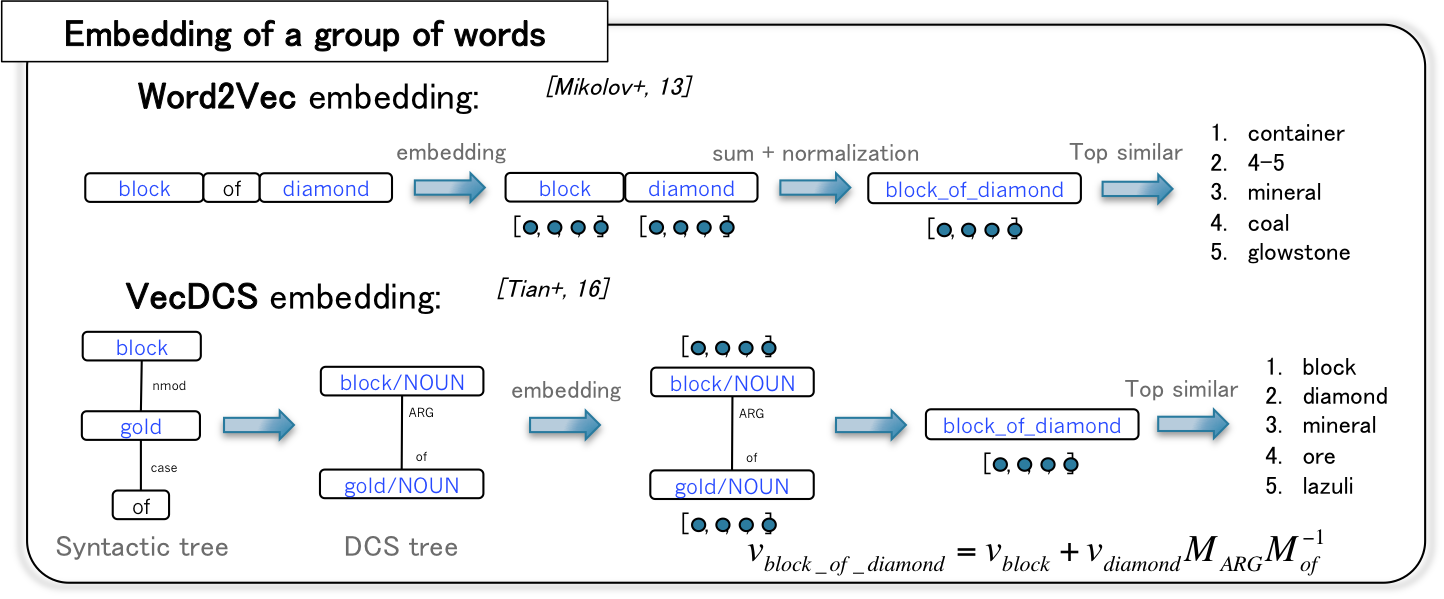
\includegraphics[width=\linewidth]{Figures/Semantic_Parsing/groupWordEmbedding.png}
   \caption{\label{groupWordEmbedding} Two phrase embedding models}
\end{figure}

Our experiment in instance classification will, then, also be a way to study the performance of each embedding model (the VecDCS model being expected to produce more effective features).

\subsubsection{Models for Instance Classification}

We defined two baseline models for the instance classification step.
The first one uses a string similarity method (we refer to it as StringSim). It does not use embedding models to classify words. We just compare the words of the phrase to classify with the names of every instance classes in the ontology, and chose the closest instance class as the prediction for the phrase. To calculate the string similarity between two phrases (the name of an instance class of the ontology is also a phrase/group of words), we use a combination of the Levenshtein distance and the Hungarian algorithm (an alignment algorithm) to align words.\\
In details (see Figure~\ref{distance}), we create a matrix with as many rows as there are words in the first phrase and as many columns as there are words in the second phrase. We add an additional row and an additional column that correspond to the empty word (so that we can align a word on the empty word and have a different number of words in the two groups). Then we fill the cells of the matrix with the Levenshtein distance between words of the two phrases. Finally, we use a variation of the Hungarian algorithm to find the alignment of words that minimize the sum of the distances. The variation allows aligning any number of words (include no word) on the empty word. The result of this Hungarian algorithm on the constructed matrix is the distance between the two phrases (see Figure~\ref{distance}). If all words are aligned on the empty word (the cost of creating a word is smaller than the transformation of a word of the other group to this word), then there is no similarity between the two phrases and the distance in set to infinite.

\begin{figure}[t]
   \centering 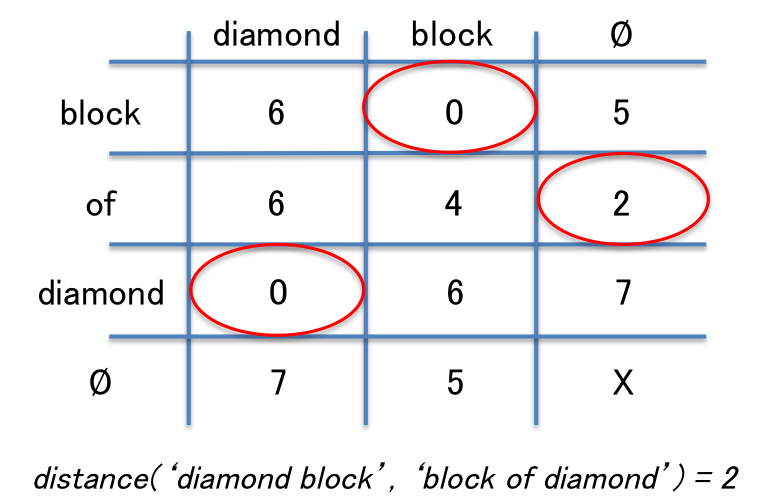
\includegraphics[width=\linewidth]{Figures/Semantic_Parsing/distance.png}
   \caption{\label{distance} Distance between 'diamond block' and 'block of diamond'}
\end{figure}

Note that even if the distance is infinite for distant phrases, we can fix a finite upper limit on the acceptable distance between a phrase to classify and the names of classes. Over this limit, or threshold, even if a class name is the closest to the phrase among all classes, the phrase will not be classified with this class. This threshold is the only parameter of the StringSim model.

The second baseline, Flat SVM model (Figure~\ref{flatSVMModel}), uses the simple Word2Vec embedding model to extract features from a phrase, and we classify the features with a multi-class RBF kernel SVM classifier that outputs one of the 508 instance classes of the ontology, or null if the group of words does not represent an instance.

\begin{figure}[t]
   \centering 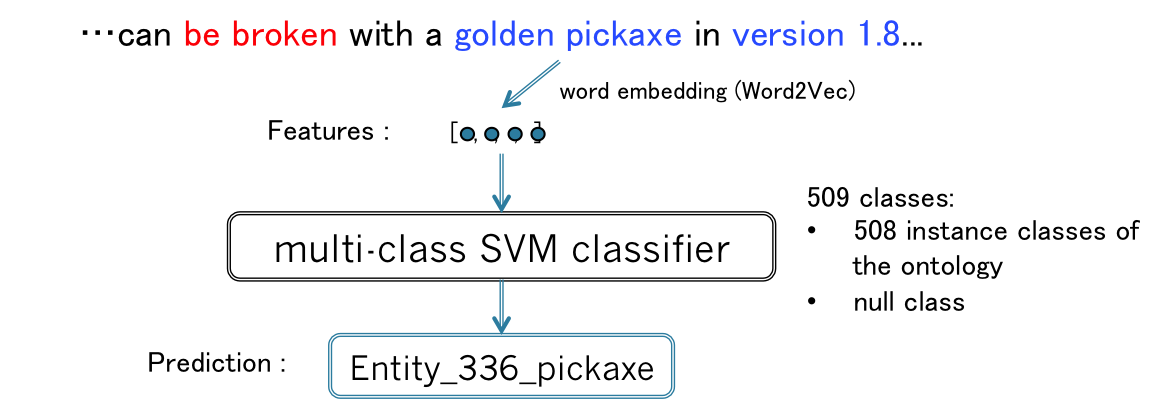
\includegraphics[width=\linewidth]{Figures/Semantic_Parsing/flatSVMModel.png}
   \caption{\label{flatSVMModel} Flat SVM model for instance classification}
\end{figure}

This model uses a C-SVC RBF kernel SVM (support vector machine) classifier implemented in the LIBSVM library \cite{chang2011libsvm} (this is also the library that we used for the other models using SVM classifiers in this work). During the training, for each class, we use positive and negative training samples. The positive samples of a class are the positive examples of the training dataset for this class and the negative samples of a class are the negative examples (not an instance) of the training dataset and the positive examples of the other classes.

Then, we defined an improved model called Hierarchical SVM model (Figure~\ref{hierarchicalSVMModel}). This is an improvement of the Flat SVM model in which we integrate the ontology's hierarchy of instances. We still use a phrase embedding model to extract features from phrases. But we do not classify the features with one multi-class SVM classifier. We classify features recursively, following the ontology's hierarchy, using one binary RBF kernel SVM classifier for each instance class. To classify a phrase, we check at first if it belongs or not to the ENTITY class and to the EVENT class, which are the two roots of the instances hierarchy, using their respective binary classifiers. If and only if it is predicted as belonging to a class, we check the belonging to the children classes (object, version, \emph{etc.}) and continue recursively. If the phrase doesn't belong to any children class, the recursion ends and the phrase is classified as the last predicted class. Note that we can obtain several predictions using this process. However, we can rank the several predictions by outputting the probabilities for each binary classifier's prediction. The probability of a prediction is defined as the geometric mean of the probabilities output by each binary classifier in the recursion. For example, in Figure~\ref{hierarchicalSVMModel}, the probability of the prediction as \textit{pickaxe} is:

\begin{quote}
$P(Entity\_336\_pickaxe) =$\\
$	(P(ENTITY)*P(object)*P(item)*P(tool)*P(pickaxe))^{1/5}$
\end{quote}

\begin{figure}[t]
   \centering 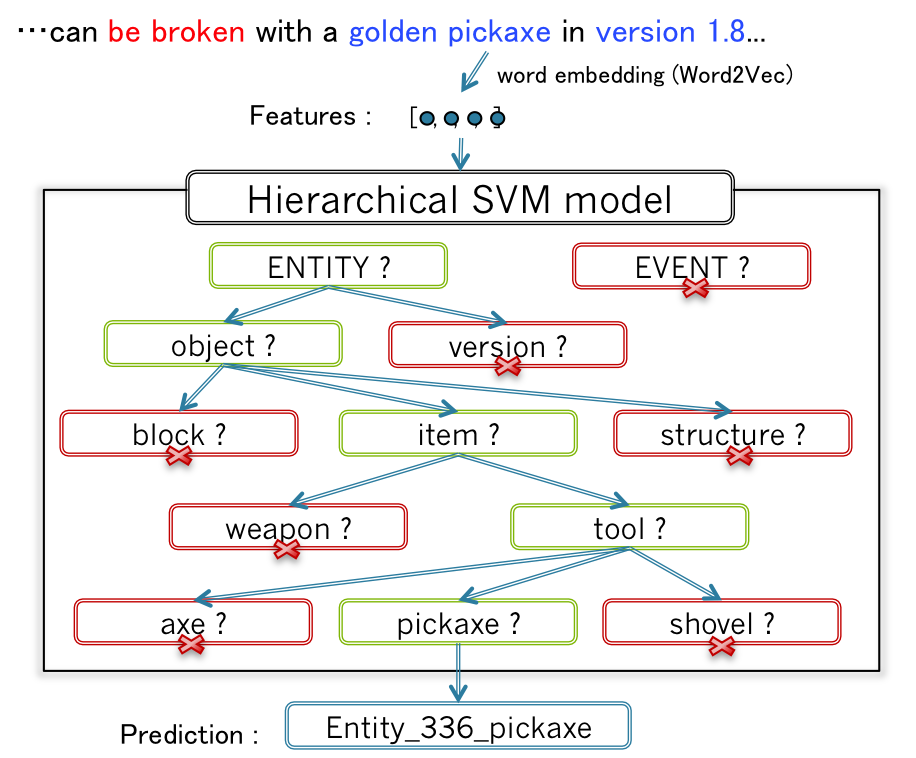
\includegraphics[width=\linewidth]{Figures/Semantic_Parsing/hierarchicalSVMModel.png}
   \caption{\label{hierarchicalSVMModel} Improvement: Hierarchical SVM model for instance classification}
\end{figure}

As for the Flat SVM model, this model uses C-SVC RBF kernel SVM classifiers. During the training, for each class, we use positive and negative training samples. The positive samples of a class are the positive examples of the training dataset for this class and for all the descendent classes in the ontology's hierarchy. The negative samples of a class are only the positive examples of the sibling classes and the direct parent classes, except for the roots of the hierarchy (ENITITY\_0 and EVENT\_0) for which the negative samples are the negative examples (not an instance) of the training dataset.

\subsubsection{Experimental results for Instance Classification}

We used the training dataset built before to train models (except StringSim that does not require training), and to test them through a 2-1 cross-validation.
We calculated the micro F1-score and the macro F1-score for each model. Results are presented in Table~\ref{resultsInstanceClassification}. The micro F1-score can be considered as the performance of the model on frequent classes and the macro F1-score gives the same importance to frequent and rare classes, so the difference between micro and macro F1-scores gives an idea of the difference of performance between frequent and rare classes.

\begin{table*}[t]
\center
\begin{tabular}{c||c|c|c|c}
	 & Micro & \multicolumn{3}{c}{Macro} \\
	Model & F1 & F1 & Precision & Recall \\
	\hline
	\hline
	strict StringSim & 0.423 & 0.810 & 0.929 & 0.719\\
	(threshold = 1) & & & & \\ \hline
	soft StringSim & 0.574 & 0.765 & 0.715 & \textbf{0.823}\\
	(threshold = 4) & & & & \\ \hline
	Flat SVM Model & 0.719 & 0.556 & \textbf{0.955} & 0.392\\
	(Word2Vec embedding) & & & & \\ \hline
	Hierarchical SVM Model & 0.791 & 0.761 & 0.801 & 0.724\\
	(Word2Vec embedding) & & & & \\ \hline
	Hierarchical SVM Model & \textbf{0.869} & \textbf{0.855} & 0.896 & 0.817\\
	(VecDCS embedding & & & & \\
	+ Word2Vec embedding of context) & & & &
\end{tabular}
\caption{\label{resultsInstanceClassification} Experimental results for Instance Classification}
\end{table*}

By comparing the two baselines (StringSim and Flat SVM model), we can see that the Flat SVM model, that uses embedding features is more performing on frequent classes, because frequent classes have more lexical diversity, and then classifying the meaning of words is better than classifying the surface of words. However, the Flat model uses only one SVM classifier for more than 500 classes, and as a result, rare classes are not correctly learnt even if this model has the best macro precision. This can be seen through its very low recall in Table~\ref{recallInstanceClassification}, or by looking at the confusion matrix of the classification in Figure~\ref{flatConfusion}.\\

\begin{figure}[t]
   \centering 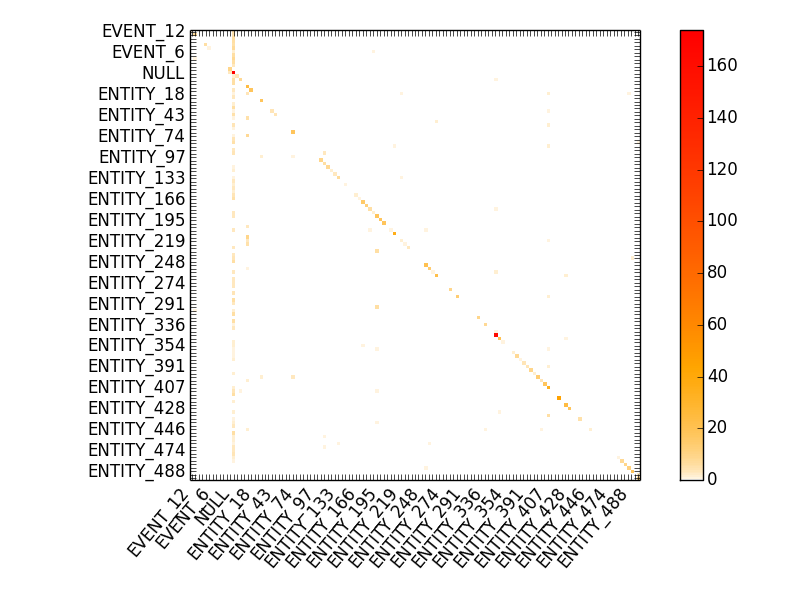
\includegraphics[width=\linewidth]{Figures/Confusion_Matrices/confusionMatrixInstanceClassificationGlobal_flat.png}
   \caption{\label{flatConfusion} Confusion matrix of instance classification with the Flat SVM model}
\end{figure}

But if we compare the Flat SVM model with the Hierachical SVM model when using the Word2Vec phrase embedding model, we can see that we make a large improvement on rare classes by using the hierarchy of instances, as the gap between micro and macro F1-score largely decreases. Still, it is not sufficient to beat the String Similarity baseline in term of macro F1-score.\\
However, we could improve the performance of the Hierachical SVM model by changing the embedding model used to extract features from the phrase to classify. Instead of using the phrase embedding model based on Word2Vec word embedding alone, we use a combination of it with the more elaborate phrase embedding model based on VecDCS word embedding. The phrase embedding model based on VecDCS is used to extract a feature vector from the phrase to classify, and the phrase embedding model based on Word2Vec is used to extract a feature vector from the context of the phrase. To do so, we apply the Word2Vec phrase embedding model on the bag of words constituted with the words located at the nodes of the syntactic tree that are directly adjacent to at least one node that is part of the phrase to classify. The concatenation of these two vectors of features is used to classify the phrase. With this model, we obtain the best performance for both micro and macro F1-scores. And if we look at the Table~\ref{recallInstanceClassification}, we can see that the good performance of the Hierarchical SVM model is due to a good balance between precision and recall.

\subsubsection{Conclusion on Instance classification}

As a conclusion on instance classification, we have shown that:
\begin{itemize}
\item Word embedding models are useful in the classification of frequent instance classes with high lexical diversity.
\item Using the ontology's hierarchy is useful to learn to classify correctly rare instance classes.
\item We can use elaborate features (VecDCS embedding features and context features) to obtain the best performance on the instance classification task.
\end{itemize}

\subsection{Relation classification}

Relation classification is the classification of the syntactic paths of a syntactic tree into relation classes from the ontology. 
Similarly to what we saw in the section on word embedding, convert syntactic paths to their vector representation could be an efficient way to produce features to classify with a SVM model.

\subsubsection{Dependency Embedding}

We need an embedding model for syntactic paths that will produce similar vector representations for similar paths. The question is then, what are similar paths?\\
As syntactic paths are sequences of words and syntactic dependencies, similar paths will be similar sequences, so it is logical to begin by embedding the elements that compose the sequences: words and syntactic dependencies. We already have a word embedding model, so we need to train a dependencyembedding model that will produce similar vectors for similar dependencies. 
Contrary to words, for which we can find synonyms, each dependency has a distinct syntactic role. However, some dependencies can be closer than others, such as $advcl:when$ (when condition) and $advcl:if$ (if condition), which are closer than $advcl:when$ and $advcl:to$ (consequence, or reversed condition). We can also notice the similarity between single dependencies and bigrams of dependencies (e.g. $nsubj$ and $nsubj\_xcomp^{-1}$), so it can be useful to be able to embed both unigrams and bigrams of dependencies.\\
To embed a dependency, or a bigram of dependencies, we used the skip-gram model implemented in the Word2Vec library (syntactic paths being composed from both words and dependencies, making our dependency embedding vectors similar to word embedding vectors simplify the implementation of the syntactic path embedding model). Training such a model only needs a corpus of dependencies sequences (in other words, syntactic paths), so we parsed a part of the knowledge corpus we extracted before with a syntactic parser, and constituted a corpus of syntactic paths. We produced two syntactic dependency embedding models, the first one embedding dependency unigrams, the other one embedding dependency bigrams. For the second one, when constructing the training corpus of syntactic paths, we divided dependency sequences by bigrams, in order to train the embedding model on bigrams of dependencies.

\begin{figure}[t]
   \centering 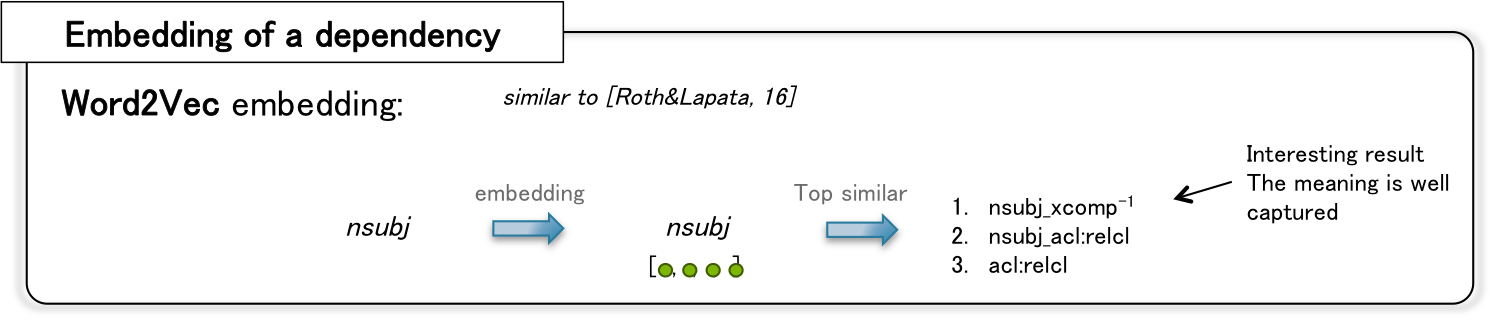
\includegraphics[width=\linewidth]{Figures/Semantic_Parsing/dependencyEmbedding.png}
   \caption{\label{dependencyEmbedding} Embedding of a syntactic dependency unigram}
\end{figure}

To construct a syntactic paths embedding model from a word embedding model and a syntactic dependency embedding model, we begin by dividing the path into two sequences, the sequence of words and the sequence of dependencies.\\
We calculate the embedding vector of the sequence of words by simply calculating the average vector of the embedding representations of all the words in the sequence (the order of the sequence is not used). For the sequence of dependencies, we calculate the average vector of the embedding representations of all dependency unigrams in the path using the first embedding model (the order of the sequence is not used), or of all dependency bigrams in the path using the second embedding model (the order of the sequence is important here).\\
Then we concatenate the embedding representation of the sequence of dependencies and the embedding representation of the sequence of words to obtain the embedding representation of the path.

\begin{figure}[t]
   \centering 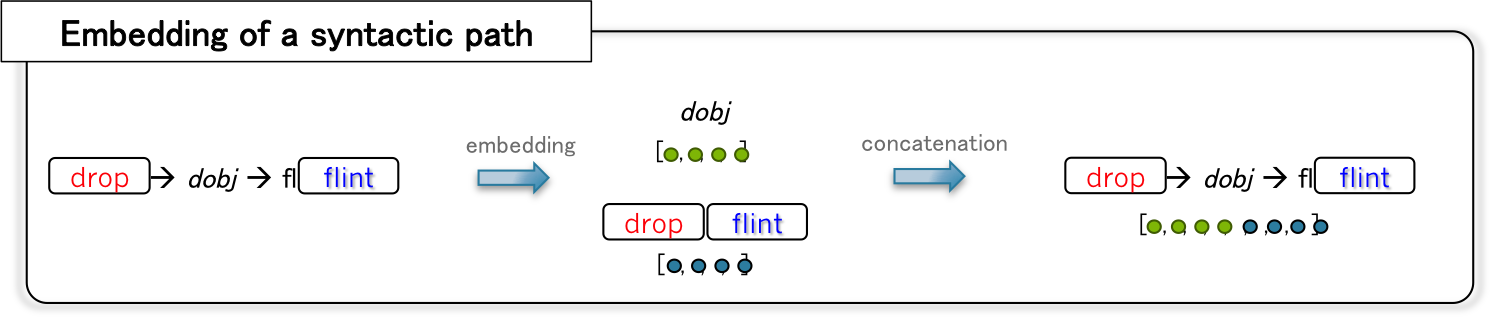
\includegraphics[width=\linewidth]{Figures/Semantic_Parsing/pathEmbedding.png}
   \caption{\label{pathEmbedding} Embedding of a syntactic path}
\end{figure}

We finally dispose of two syntactic path embedding models, one that uses dependency unigram embedding and does not encode the order of the sequence, and an other that uses dependency bigram embedding and then integrates the order of the sequence of dependencies in the syntactic path. If our purpose is similar to the syntactic path embedding done in the work of M. Roth and M. Lapata in 2016 \cite{roth2016neural}, the technology used to construct the model in different. It would then be interesting to compare both approaches in a future work.\\
In our syntactic path embedding models, we also added the possibility not to consider the words in the syntactic path, in which case the path embedding models only embed the sequence of dependencies (unigrams or bigrams).

\subsubsection{Models for Relation Classification}

First, we created a baseline that uses one binary SVM classifier for each relation of the ontology, including the root RELATION of all relations (see Figure~\ref{relationClassificationBaseline}).
After extracting the features from the syntactic path we want to classify with our path embedding model, we begin by testing if the path represent or not a relation of our ontology by classifying it with the root RELATION binary classifier. If the root relation's classifier prediction is positive, we test for each relation class in the ontology if the path belongs to the class or not by using the respective binary SVM classifiers (the classification is then similar to the Hierarchical SVM model for instances in the case of events that have no other hierarchy that the common root). In the example of Figure~\ref{relationClassificationBaseline}), only the \textit{ingredient} relation class is predicted positively.

\begin{figure}[t]
   \centering 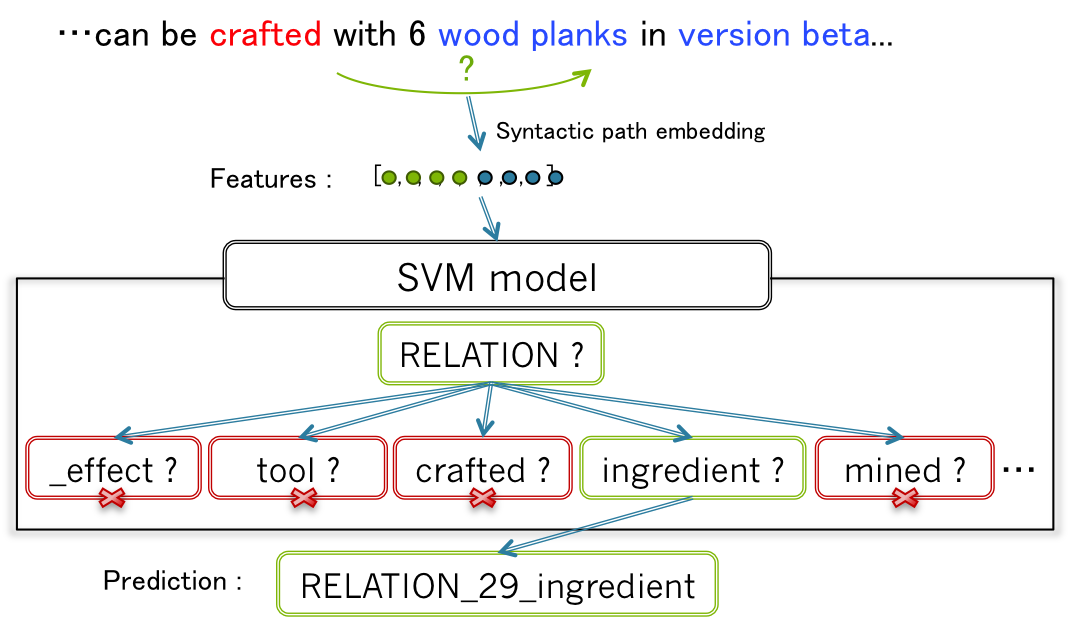
\includegraphics[width=\linewidth]{Figures/Semantic_Parsing/relationClassificationBaseline.png}
   \caption{\label{relationClassificationBaseline} SVM model for relation classification}
\end{figure}

During the training, for each class, we use positive and negative training samples. In the case of the root relation binary classifier, we use all positive examples of the training dataset as positive samples, and all negative examples of the training dataset as negative samples. However, for any other class, the positive samples are the positive examples of the training dataset for this class and the negative samples are the positive examples of the other classes. Using a classifier for the root relation as a first step of the classification instead of testing directly all the relation classes is a way the reduce the number of predictions done by SVM classifiers, and it allows to train relation classes with less negative samples, as the non-relation paths are eliminated by the root classifier at the first step.

We built an improvement of the previous model, by integrating the ontology's constraints into the model (see Figure~\ref{relationClassificationImprovement}).
Indeed, constraints provide useful information when classifying a relation, so we added a constraints verification step at the top of the model.
In other words, before classifying the features of a syntactic path between two entities, we check what relation classes are possible candidates for the relations between these two instances. In the example of Figure~\ref{relationClassificationImprovement}, a relation between ``crafted'' and ``wood planks'' cannot be \textit{\_effect} or \textit{type\_of}, but only \textit{crafted} or \textit{ingredient}. So it is theoretically useless to check if the syntactic path belong to other classes than \textit{crafted} and \textit{ingredient}.

\begin{figure}[t]
   \centering 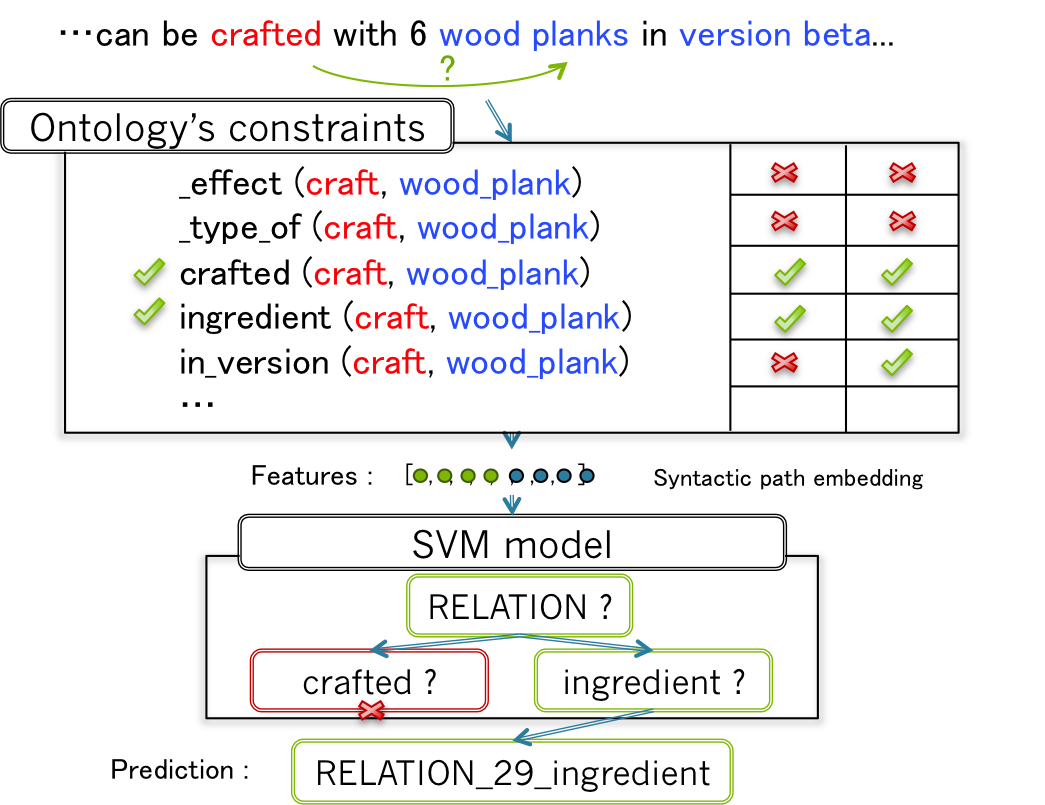
\includegraphics[width=\linewidth]{Figures/Semantic_Parsing/relationClassificationImprovement.png}
   \caption{\label{relationClassificationImprovement} Improvement: SVM model with constraints for relation classification}
\end{figure}

As for the baseline, during the training, for any class except the root, the positive samples are the positive examples of the training dataset for this class, however the negative samples are only the positive examples of the other classes for which this class was also a candidate. The constraints verification step then allows to reduce the number of negative samples even more, which speeds up the training.\\
For each of the two models, we can use either the unigram-based syntactic path embedding model or the bigram-based syntactic path embedding model to produce the features to classify, and for each embedding model, we can consider or not the words of the syntactic paths. In the following section, we will compare both models, but also the difference in performance for each model depending on the syntactic path embedding model that is used to extract features.\\
Such as the Hierarchical SVM model for instance classification, both relation classification models use C-SVC RBF kernel SVM classifiers.

\subsubsection{Experimental results for Relation Classification}

We used the training dataset built before to train and to test our relation classification models (through 2-1 cross-validation). The result of this experiment in presented in Table\ref{resultsRelationClassification}.

\begin{table*}[t]
\center
\begin{tabular}{c||c|c|c|c}
	 & Micro & \multicolumn{3}{c}{Macro} \\
	Model & F1 & F1 & Precision & Recall \\
	\hline
	\hline
	SVM Model & 0.496 & 0.447 & 0.444 & 0.450\\
	no constraints, dependency unigrams & & & & \\ \hline
	SVM Model & 0.501 & 0.456 & 0.474 & 0.440\\
	no constraints, dependency bigrams & & & & \\ \hline
	SVM Model & 0.767 & 0.789 & \textbf{0.884} & 0.713\\
	constraints, dependency unigrams & & & & \\ \hline
	SVM Model & \textbf{0.792} & \textbf{0.791} & 0.871 & \textbf{0.725}\\
	constraints, dependency bigrams & & & & \\ \hline
	SVM Model & 0.702 & 0.638 & 0.862 & 0.506\\
	constraints, words and dependency bigrams & & & &
\end{tabular}
\caption{\label{resultsRelationClassification} Experimental results for Relation Classification}
\end{table*}

This experiment confirms the positive impact of using constraints of the ontology in the relation classification model. Indeed, using constraints reduces the number of possible labels, so it also reduces the number of possible classification errors. The improvement is largely visible by comparing the confusion matrices of the models without and with constraints (Figure~\ref{relationConfusion})\\
An other interesting result is that using a constraints verification step in the model implies that we do not need to train the binary SVM classifiers by using the samples of other relation classes as negative samples if the two relations do not link the same instance classes. This results in a faster training, as we reduce the number of negative samples that are necessary.\\
We can also observe that using the bigram-based syntactic path embedding model to extract the features slightly increases performance, which shows that the order in the sequence of dependencies is important.\\
However, using both the words and the syntactic dependencies of the path to classify in the features is less performing than using the dependencies only. This can be explained by two factors. First, we are considering here the constrained SVM model in which the number of candidates in the classification in very limited. Such a small number of possible candidates may explain that the dependencies alone are sufficient to make the distinction between these few candidates, and it may be the reason why performance does not increase when using the words of the path. Secondly, we are working with very low resource, and our training set is small. Then, there may be enough samples to learn the typical syntax used by each relation, but not enough to learn the diversity of words that can be used with this syntax. A further study with a larger training dataset might show some improvements in using words in the syntactic paths classification, but as our purpose is to work with low resource, this result encourages to develop models that use the information of words more efficiently, without a need to increase the size of the training dataset.\\
Looking at the Table\ref{recallRelationClassification}, we can see that the main weakness of our relation classification models is the low recall of the process. As we are working with low resource and few training samples, making improvements on the recall without increasing the number of costly expert annotations would be valuable. We will see in the next section how we can increase the size of the training dataset without doing expert annotations of relations by using crowd-sourcing.\\

\begin{figure}[t]
   \centering
   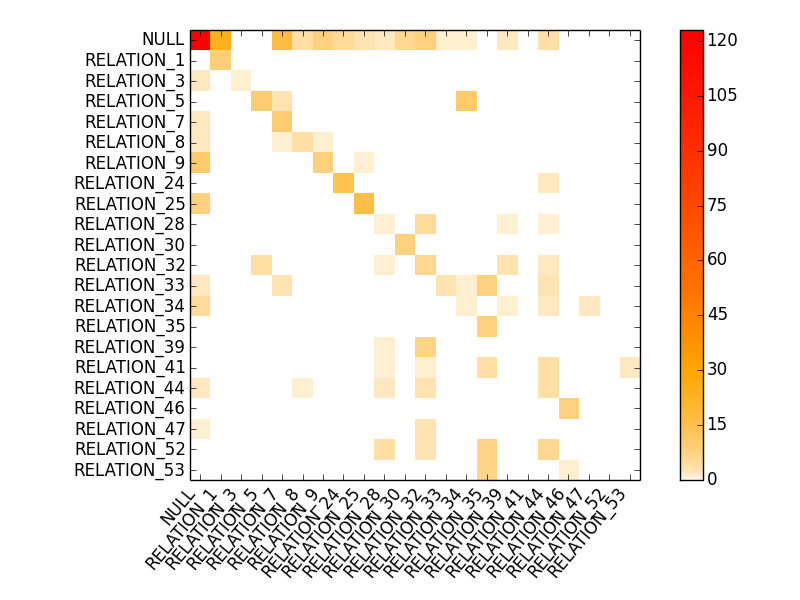
\includegraphics[width=0.5\linewidth]{Figures/Confusion_Matrices/confusionMatrixRelationClassification_noConstraints.png}\hfill
   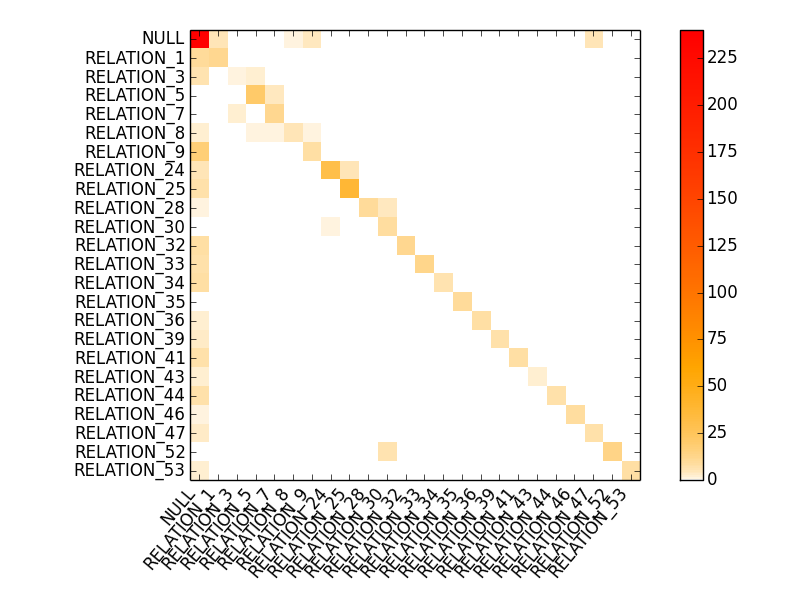
\includegraphics[width=0.5\linewidth]{Figures/Confusion_Matrices/confusionMatrixRelationClassification_constraints.png}
   \caption{\label{relationConfusion} Confusion matrices of relation classification using dependency bigrams features without constraints (left) and with constraints (right)}
\end{figure}

We also evaluated the quality of the annotated data by comparing the performance of the relation classification cross-validation on the crowd-sourcing annotations to the performance of cross-validation on expert annotations (see Table~\ref{crowdSourcingRelationClassification}).

\begin{table*}[t]
\center
\begin{tabular}{c||c|c}
	Model & Micro F1 & Macro F1 \\
	\hline
	\hline
	SVM Model & & \\
	constraints, dependency bigrams & \textbf{0.792} & \textbf{0.791} \\
	(expert annotations only) & & \\ \hline
	SVM Model & & \\
	constraints, dependency bigrams & 0.763 & 0.719 \\
	(crowd-sourcing only) & & \\ \hline
	SVM Model & & \\
	constraints, dependency bigrams & 0.780 & 0.754 \\
	(expert + crowd-sourcing) & &
\end{tabular}
\caption{\label{crowdSourcingRelationClassification} Relation Classification performance on crowd-sourcing annotations}
\end{table*}

If the performance of the cross-validation on crowd-sourcing annotations is slightly below the performance on expert annotations, we can nonetheless conclude that crowd-sourcing can be a good way of increasing the size of the training dataset for relation classification when using the annotating method described before to make the annotation accessible to non-expert annotators.

We made a further experiment to show the impact of the quality of the syntactic information that is classified. We saw that our relation classification models classify syntactic paths that are obtained from sentences with syntactic parsers. In this experiment, we use the same relation classification model (SVM model with constraints, using either dependencies unigrams or bigrams, but not words) and the same training dataset, but we use two different syntactic parsers to obtain the syntactic paths from which we extract the features to classify (see Table~\ref{impactSyntaxRelationClassification}).

\begin{table*}[t]
\center
\begin{tabular}{c||c|c}
	Model & Micro F1 & Macro F1 \\
	\hline
	\hline
	SVM Model & & \\
	with constraints, dependency unigrams & 0.767 & 0.789 \\
	(\textit{Parsey McParseface} Parser) & & \\ \hline
	SVM Model & & \\
	with constraints, dependency bigrams & \textbf{0.792} & \textbf{0.791} \\
	(\textit{Parsey McParseface} Parser) & & \\ \hline
	SVM Model & & \\
	with constraints, dependency unigrams & 0.731 & 0.774 \\
	(\textit{Stanford} Parser) & & \\ \hline
	SVM Model & & \\
	with constraints, dependency bigrams & 0.774 & 0.784 \\
	(\textit{Stanford} Parser) & &
\end{tabular}
\caption{\label{impactSyntaxRelationClassification} Impact of the syntactic information quality on Relation Classification performance}
\end{table*}

The two parsers we use are the Stanford Parser \cite{chen2014fast} and the Parsey McParseface Parser \cite{andor2016globally}; the last one have been shown to achieve state-of-the-art performance on the syntactic parsing task.\\
As a result, we observe a significant difference in the performance of the relation classification model, with better performance when using the Parsey McParseface parser to obtain the syntactic paths. This is mainly due to the fact that even a small difference in the syntactic tree of a sentence can lead to big changes in the syntactic paths and make them more difficult to classify correctly with our relation classification models. Therefore, using a syntactic parser that avoid mistakes has a significant positive impact on the relation classification model's performance.

\subsubsection{Conclusion on Relation classification}

As a conclusion on relation classification, we have shown that:
\begin{itemize}
\item A dependency embedding model can be trained from the extracted corpus (after parsing it with a syntactic parser) and allows to classify syntactic paths.
\item Using the ontology's constraints increases performance and speed up the training.
\item Using dependency bigrams instead of unigrams, and then taking into account the order of the dependencies in the syntactic path slightly increases performance.
\item Using both words and dependencies from the paths to classify decreases performance, which shows that we must re-think the way we are using the word information in the path classification.
\item The quality of the crowd-sourcing annotations is close to the quality of expert annotations.
\item The quality of the syntactic information that we classify in the Relation classification step has a significant impact on performance.
\end{itemize}

\section{Discussion}

%In this work, we presented a study about semantic parsing with very low annotated resource in the domain of the video game Minecraft. We have shown that such a semantic parser can be performing in the restricted domain if we make good use of the data we created, in particular by using the ontology's characteristics, and that it can be trained with only a few manually annotated resource and can be completed with automatically generated samples or through crowd-sourcing annotations.\\
%The main contribution of our study when compared to other works describing methods to build semantic parsers for limited domains \cite{wang2015building} is that we explored various ways to increase the parsing performance by acting on both the size of the training dataset with several methods (web anchors, crowd-sourcing), and the classification models (integrating ontology in the classification step and extracting relevant features).\\
%Thus, we believe that our work is then a first step in answering to how to efficiently build a semantic parser with very low resource and use it to do advanced question answering in restricted domains.\\
%As future works, we believe that some work should be done to improve the relation classification step of the semantic parsing. Indeed, the recall still has to be reduced, which implies a lot of manual annotations with the current methodology. One interesting problematic could be to answer the question: can we create training data automatically from available resource, as we did with anchors for instance classification? We could for example imagine using distant supervision to create automatically relations samplesfrom the structured relations of the web infoboxes.\\
%We think that some work should also be done to reduce even more the quantity of manual work needed to build the ontology of the restricted domain. There have been some interesting works on how a system can learn to produce knowledge graphs without any ontology \cite{hixon2015learning} that have shown that the performance are particularly good in restricted domains. Or may even be possible to limit semantic parsing to instance classification and do question answering directly on syntactic trees \cite{gomez2014graph}.
%Then, a study should be done on the application of the knowledge graphs produced by semantic parsing on question answering in Minecraft. Finally, it would be interesting to use our models to train and test a semantic parser and a QA system on other low resource restricted domains \cite{molla2007question} such as technical fields (medical domain, industrial domains, \emph{etc.}), customer services, or other video games.

%----------------------------------------------------------------------------------------
%	REFERENCE LIST
%----------------------------------------------------------------------------------------

\bibliography{references}
\bibliographystyle{apalike}

%----------------------------------------------------------------------------------------

\end{document}
